%FW
%Fixing the current solution
    %Commercialize
        %Usability issues to address
        %System Stability & Performance
            %Real NTP
            %MediaCodec
        %Multiple Device Crash
            %WiFi-Direct
        %Psychoacoustics are currently not explicitly utilized, need more sync control
%Expanding further
    %Surround System, PCM per channel
    %Actually use psychoacoustics
    %What are the possibilities with psychoacoustics?
\section{Future Work}
\author{Marc}
\begin{frame}{Future Work}
    \framesubtitle{Overview}
    \begin{itemize}
        \item{Improving the Application}
        \begin{itemize}
            \item Fixing Critical Issues
            \item Improving Stability \& Performance
            \item Commercializing the Application
        \end{itemize}
        \item{Expanding the Application}
        \begin{itemize}
            \item Surround System
            \item Psychoacoustics
        \end{itemize}
    \end{itemize}
\end{frame}

\subsection{Improving the Application}
\begin{frame}{Improving the Application}
    \framesubtitle{Fixing Critical Issues}
    \begin{description}
        \item [Issue] We are unable to connect more than one slave.
        \item [Cause] Yet unknown.
        \item [Solution] Use an alternative to WiFi-Direct, this would also solve the future problem of relatively low device limit. %Currently best known alternative would be NearbyConnections API
        %Client to service connection shuts down if screen goes off - doesnt work as a started service is supposed to - acts like a bound service.
    \end{description}
\end{frame}

\begin{frame}{Improving the Application}
    \framesubtitle{Fixing Critical Issues}
    \begin{description}
        \item [Issue] When the screen of a slave is shut down, it stops playing.
        \item [Cause] The network connection to the master is terminated due to not handling Android processes properly.
        \item [Solution] We need to introduce wakelocks and persistent notifications for the network to keep the data stream alive.
    \end{description}
\end{frame}

\begin{frame}{Improving the Application}
    \framesubtitle{Improving Stability \& Performance: Synchronization}
    \begin{description}
        \item [Area of the system] Our SNTP approach to \textit{clock synchronization}.
        \item [Cause for subpar solution] The alternative is complex, time consuming and imposes restrictions.
        \item [Possible improvement] Implementing NTP.
        \item [Benefit] More \textit{consistent} synchronization and alleviation for drift.
        %More consistant sync, refer to Troels' stuff
    \end{description}
\end{frame}

\begin{frame}{Improving the Application}
    \framesubtitle{Improving Stability \& Performance: Occasional Crashes}
    \begin{description}
        \item [Area of the system] Audio data management throughout the system.
        \item [Cause for subpar solution] Unaware of possible solutions that have later come to light.
        \item [Possible improvement] Android has a range of APIs that possibly can handle decoding of audio, data transferring and media synchronization, namely \textit{MediaCodec} and \textit{MediaSync}
        %Jesper talks about these i believe, ref back
        \item [Benefit] Could possibly fix \textit{stability} issues causing crashes.
        %Our theory is that this is caused by bad handling of \textit{audio buffers}, using tested APIs may help solve this.
    \end{description}
\end{frame}

\begin{frame}{Improving the Application}
    \framesubtitle{Commercializing the Application: Music Source}
    \begin{description}
        \item [Current Approach] Only \textit{local} MP3 files are available.
        \item [Improved Approach] Implementing API support for a larger \textit{streaming} service with access to music.
        \item [Why it is required] Most music today is streamed.
        %as such for the application to see actual use it needs access to music, and while there may exist local music, this would be sparse and slaves would not be able to queue or suggest music.
    \end{description}
\end{frame}

\begin{frame}{Improving the Application}
    \framesubtitle{Commercializing the Application: Media Control}
    \begin{description}
        \item [Current Approach] Only simple constructs such as pause, play, next, previous and auto play features exist.
        \item [Improved Approach] Playlists and a queue/suggestion system.
        \item [Why it is required] To have some \textit{control} over the music without constant management.
    \end{description}
\end{frame}

\begin{frame}{Improving the Application}
    \framesubtitle{Commercializing the Application: Usability}
    \begin{description}
        \item [Current Approach] Functional.
        \item [Improved Approach] A UI needs to be designed, implemented and tested, supporting the aforementioned improvements required to commercialize the application.
        \item [Why it is required] It matters little what the application can do, if it is not \textit{approachable} and easy to use by users.
    \end{description}
\end{frame}

\subsection{Expanding the Application}
\begin{frame}{Expanding the Application}
    \framesubtitle{Surround System}
    \begin{description}
        \item [Idea] Each device acts as a speaker
        \item [Challenge] The devices need to know their relative location to target.
        \item [Challenge] The master has to distribute the right channels to the right devices.
        \item [Challenge] Devices can leave the system without telling others, how to replace/adjust?
    \end{description}
\end{frame}

\begin{frame}{Expanding the Application}
    \framesubtitle{Psychoacoustics}
    \begin{description}
        \item [Idea] Actively utilize psychoacoustics %we dont atm, it saves our hide currently
        \item [Challenge] We need very reliable synchronization.
        \item [Challenge] Knowledge of the devices relative location, speaker direction and volume.
        \item [Challenge] Other psychoacoustic effects than precedence effect may have even more specific needs.
    \end{description}
\end{frame}

\begin{frame}{Expanding the Application}
    \framesubtitle{Psychoacoustics}
    \begin{figure}
    \centering
    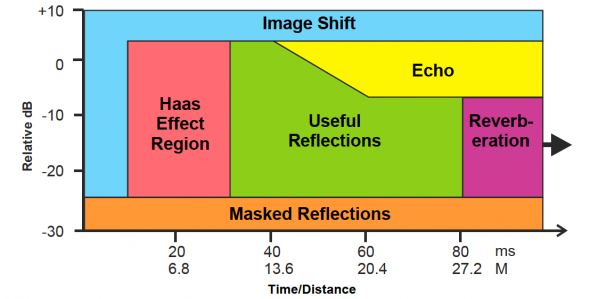
\includegraphics[height=0.5\textheight]{images/haas.png}
    \caption{source: \texttt{https://www.prosoundtraining.com/2010/03/15/its-about-time-the-effective-haas-effect/}}
    \end{figure}
\end{frame}
